\chapter{Research Path Overview}
\label{chap:intro}

Artificial intelligence (AI) is currently the buzzword on everybody's lips.
Riding the wave of recent groundbreaking achievements, from self-driving cars \cite{} to intelligent chatbots \cite{}, AI is transforming industries and reshaping our daily lives.
Several interpretations and definitions have been provided over the years, yet the seminal perspective given by the Turing test \cite{turing1980computing} is still one worth mentioning.
\begin{definition}[Artificial Intelligence \cite{turing1980computing}]
A machine that shows intelligence indistinguishable from that of human beings is qualified to be labeled as artificial intelligence.
\end{definition}
This translates into understanding what falls under the umbrella of \textit{intelligence}, which is defined differently across the research areas as reasoning, planning, and learning.
\begin{definition}[Machine Learning \cite{samuel2000some}]
A machine with the ability to learn without being explicitly programmed.
\end{definition}
Building upon the notion of intelligence as learning, i.e. Machine Learning (ML), emerged as the pinnacle of AI due to its disruptive advancements.
At its core, ML aims at addressing problems for which the development of algorithms by humans is not feasible, because the algorithm itself is either not known or cost-prohibitive.
Examples include face recognition, fraud detection, sale forecasting, and object ranking.
The problems are solved instead by letting the algorithms (e.g., neural networks \cite{nn}) \textit{discover their own solutions}: they perform a training process atop a sample of historical data, borrowing techniques from disciplines such as numerical analysis, statistics, and information theory.
The training process consists of fitting internal parameters (e.g., weights and bias) and providing practitioners with a model.
In this context, we can hence define an \textit{AI system} as the (software) solution that deploys an ML model specific for the problem at hand i.e., ready to ingest new data and tackle it.

There exists a plethora of different algorithms solving the same problem with different strengths and weaknesses, confirming theoretical results proving that there is \textit{no silver bullet} \cite{kerschke2019automated}---no algorithm dominates all others in all respects.
Besides, algorithms often expose some hyperparameters controlling the learning behavior (e.g., learning rate).
To unleash the full potential of ML, practitioners have to carefully tune such hyperparameters but get easily overwhelmed by the showcased problem of combined algorithm selection and hyperparameter (CASH) optimization.

Automated machine learning (AutoML) demonstrates to play a crucial role in this landscape by tackling the CASH problem and, going beyond, by handling ever-larger search spaces in surprisingly small time budgets \cite{small_time_budgets}.
Remarkable milestones include bayesian optimization (BO) to explore promising configurations based on prior evaluations,
meta-learning (i.e., learning atop learning) to warm-start BO (i.e., to boost the convergence process) by suggesting configurations that worked well in previous similar cases, and multi-fidelity methods to partially evaluate time-consuming configurations.
By lowering the barrier of access, AutoML emerged as promising for the democratization of AI, i.e. making it accessible to both experts and non-experts alike.
Yet, when it comes to real-case scenarios, the journey of
delivering AI systems is riddled with challenges.

\begin{figure}
    \centering
    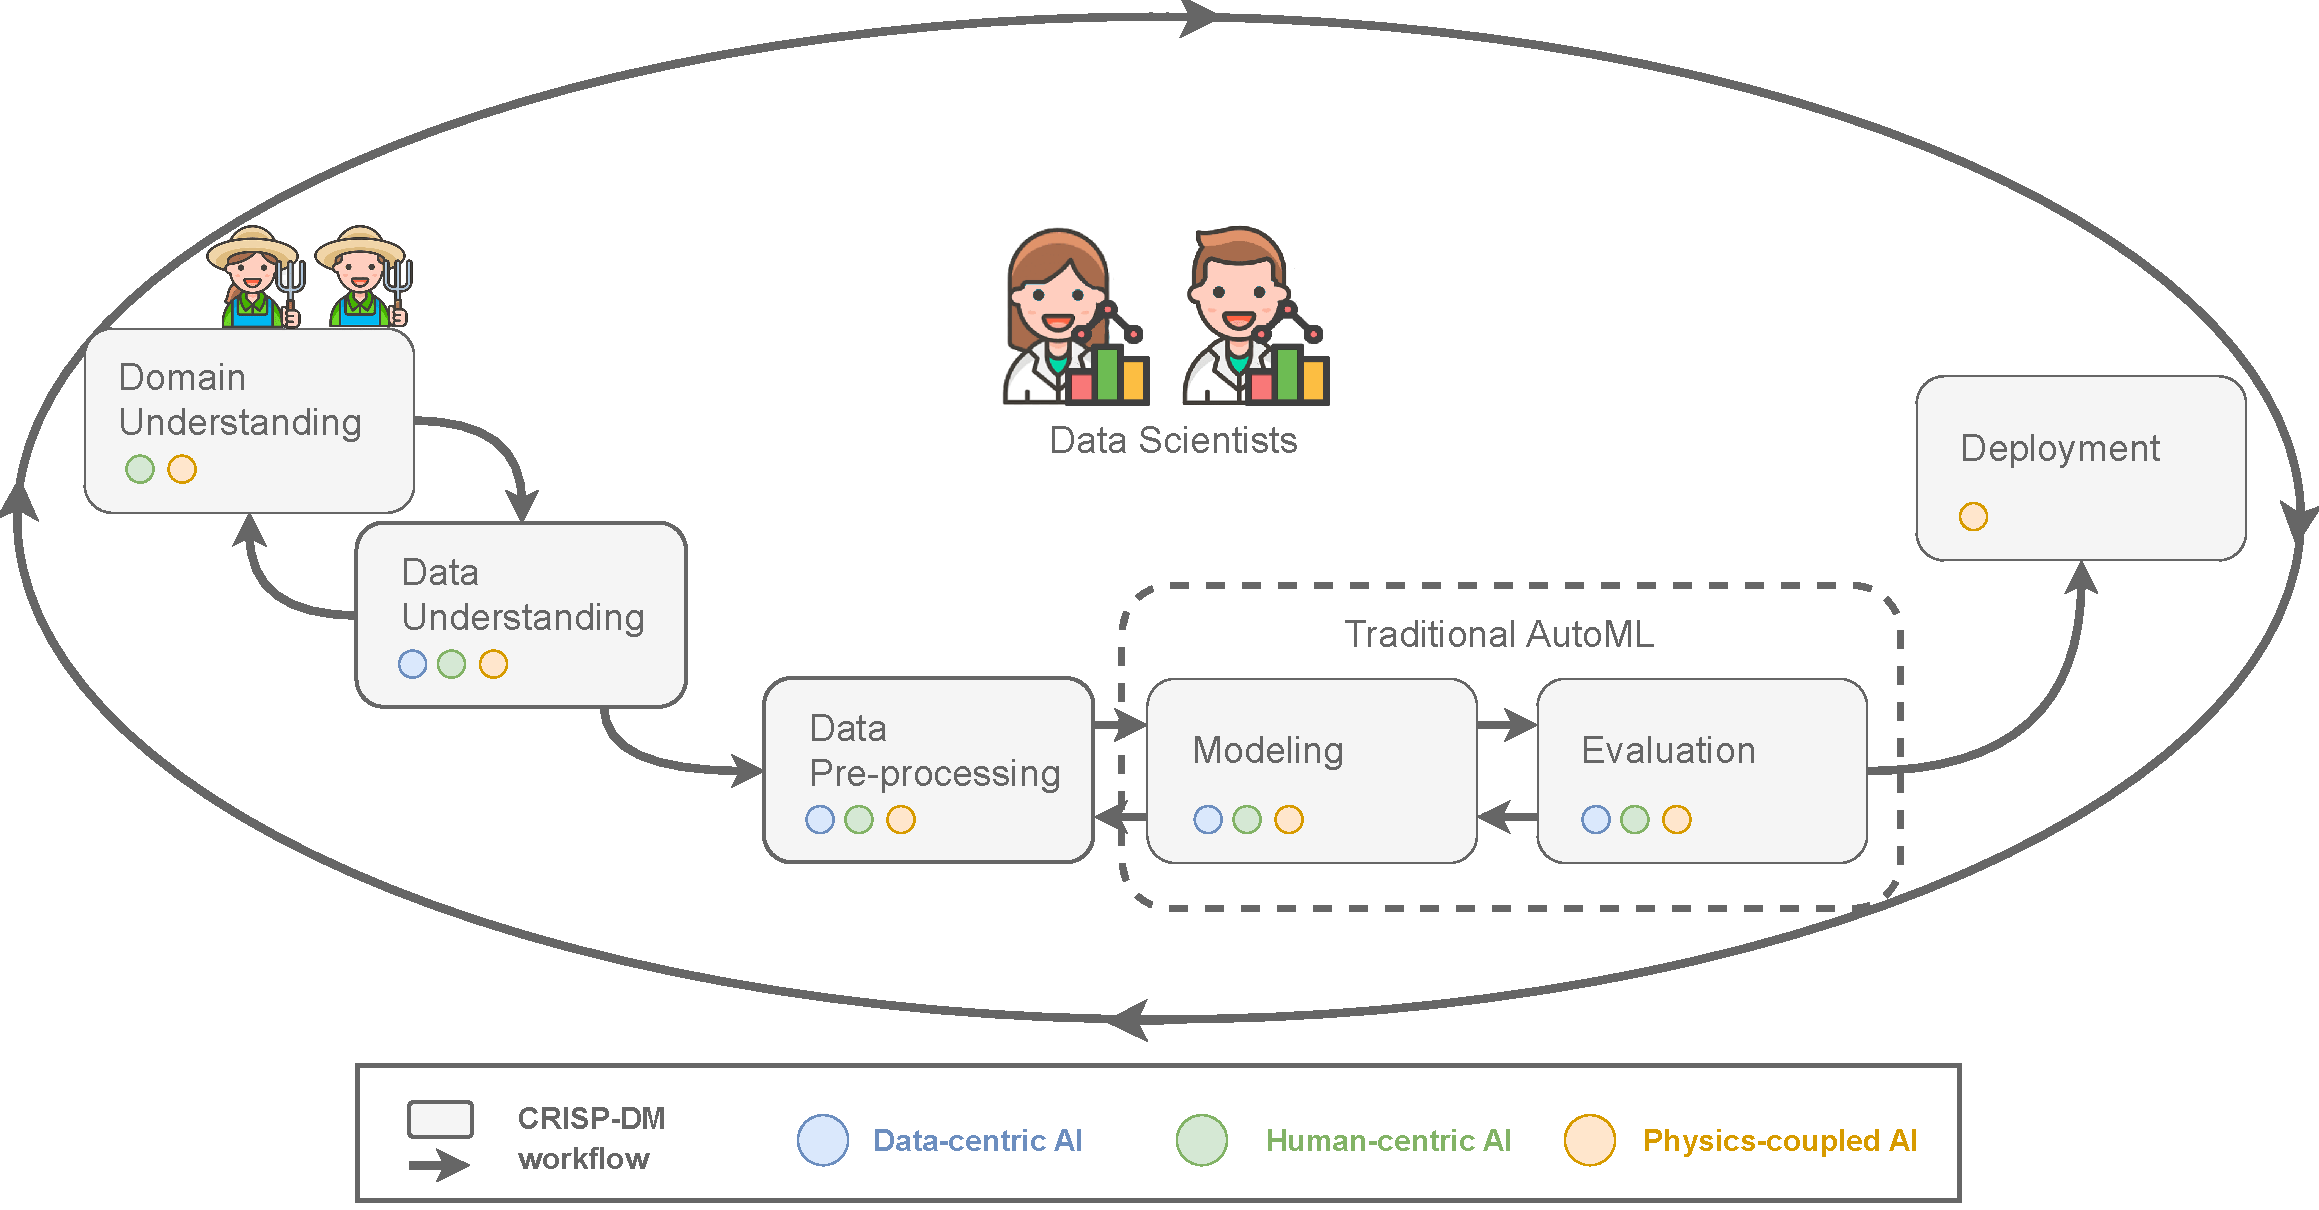
\includegraphics[scale=0.3]{chapters/introduction/img/contribution_overview.pdf}
    \caption{Contirbution Overview.}
    \label{fig:contribution}
\end{figure}

Let us quickly overview the end-to-end process.
The main character is usually the data scientist, a specialist in machine learning and data analysis, which leverages a process model to translate the \textit{knowledge} about the problem into \textit{ML constraints} and deploy the system.
The cross-industry standard process for data mining \cite{wirth2000crisp} (CRISP-DM) is considered the open standard and we will take it as a reference in the whole thesis.
Given the numerous skills expected by data scientists,
their numbers fall short of the needs,
leading domain experts to carry out such a process.
For the sake of simplicity, we keep these two roles separated.
\textbf{Domain} and \textbf{data understanding} entail domain experts and the data scientist working in close cooperation to explore constraints and study available data, respectively.
These stages might be repeated many times until the data scientists are satisfied with the acquired knowledge.
Follows the iterative investigation of different solutions throughout \textbf{data pre-processing}, \textbf{modelling}, and \textbf{evaluation}.
Data pre-processing and modelling are conducted to build a data pipeline and train an ML algorithm, respectively.
More in detail, a series of pre-processing transformations shape the data so that the ML algorithm can output the best model.
Then, evaluation offers a way to measure the performance and the process can conclude with the \textbf{deployment} of the AI system, including the implementation of the running environment.

\Cref{fig:contribution} shows the CRISP-DM process model and the research areas we focus on.
Specifically, according to challenges that are addressed: data-centric, human-centric, and physics-aware AI.
While \Cref{chap:background} provides the necessary background, the remaining of the thesis evolves in the corresponding three parts.

\section*{Part I: Data-centric AI}

During the past few decades, most of the efforts in AI were focused on improving ML algorithms, leading to numerous groundbreaking achievements.
In many applications, modelling is considered the solved part of the puzzle and the vast majority of the time is spent on improving the data.
Data-centric AI is the discipline of systematically engineering data used to build an AI system, yet the challenge of configuring data pipelines is rather simple.
A combinatorial space has to be explored, entailing ad-hoc pre-processing for the algorithm at hand, and constraints within data, transformations, and algorithms exacerbate the problem at hand.
While AutoML traditionally neglected data quality and pre-processing, there is an untapped potential to contribute to this research area.
Indeed, given the huge combinatorial space, AutoML can help in designing efficient AI systems with a meticulous focus on data.

In \Cref{part:data-centric}, we devise data-centric solutions for the main categories of ML i.e., supervised and unsupervised learning.
Specifically, we focus on the following challenges and contributions.

\subsection*{Effective Data-preprocessing Pipelines in Supervised Learning}

\paragraph{Challenge} Data pre-processing
encompasses a broad range of transformations that span from correcting errors to selecting the most relevant features for the modelling phase.
In supervised learning, during modelling, the ML algorithm is provided with ground truth to drive the learning toward a user-specified objective function.
There is no clear evidence, or rules defined, on how these transformations impact the final results of the process.
Besides, the problem is exacerbated when transformations can be combined into pipelines.
Data scientists cannot easily foresee the overall impact, requiring a method to discriminate between them and hence find the most relevant ones for their study at hand.

\paragraph{Contribution} In \Cref{data-centric-chap:supervised}, we study the impact of transformations in general, and the impact of transformations when combined together into pipelines.
We make use of rules that enable the construction of prototypes (i.e., ordered series of transformations) and, once found, these prototypes can be tuned -- similarly to algorithm hyperparameters -- using AutoML.
The optimization of our effective prototypes provides results that compared to an exhaustive search, get 90\% of the predictive accuracy in the median, but with a time cost that is 24 times smaller.

\subsection*{Exploring Clustering Pipelines via AutoML and Diversification}


\paragraph{Challenge}
AutoML has witnessed effective applications in the field of supervised learning -- mainly in classification tasks --  where the goal is to find the best ML pipeline when a ground truth is available.
This is not the case for unsupervised tasks that are by nature exploratory and they are performed to unveil hidden insights.
Since there is no right result, analyzing different configurations is more important than returning the best-performing one.
When it comes to exploratory unsupervised tasks -- such as cluster analysis --  different facets of the datasets could be interesting for the data scientist; for instance, data items can be effectively grouped together in different subspaces of features.

\paragraph{Contribution}
In \Cref{data-centric-chap:unsupervised}, we design a framework that explores and returns a dashboard of both relevant and diverse clusterings via AutoML and diversification.
AutoML ensures that the explored pipelines for cluster analysis (including pre-processing steps) compute good clusterings.
Then, diversification selects, out of the explored clusterings, the ones conveying different clues to the data scientists.

\section*{Part II: Human-centric AI}

The original promise of AutoML was to automate certain ML tasks to a significant extent, thereby democratizing it and enabling non-experts to apply it in their respective domains.
However, despite their success, many current AutoML tools were -- yet another time -- not built around the user but rather around algorithmic ideas.
The stacking of complex mechanisms on top of each other unavoidably led to a less understanding of the process -- even by ML experts -- and allowing for very limited interaction.
Parts of the community have hence pushed towards a more human-centric AutoML process aimed at complementing, instead of replacing, human intelligence.
Besides, motivated by ethical concerns and social bias issues arising at each step of the ML process, this approach becomes even imperative in such a mitigating call nowadays.
By placing the user back in the loop, we let the user to revise and supervise the entire process, ensuring fairness, transparency, and ethical compliance.

In \Cref{part:human-centric}, we focus on the following challenges and contributions.

\subsection*{Human-centric AutoML via Structured Argumentation}

\paragraph{Challenge} In the last decade, we have witnessed exponential growth in both the complexity and the number of ML techniques; leveraging such techniques to solve real-case problems has become difficult for Data Scientists.
Automated Machine Learning (AutoML) tools have been devised to alleviate this task, but easily became as complex as the ML techniques themselves---with Data Scientists losing control over the process.

\paragraph{Contribution} In \Cref{human-centric-chap:hamlet}, we design HAMLET (Human-centric AutoMl via Logic and argumEnTation), a framework that helps data scientists to redeem their centrality.
HAMLET enables data scientists to express ML constraints in a uniform human- and machine-readable medium.
User-defined constraints are interpreted to drive the exploration of ML pipelines (i.e., data pre-processing transformations shape the data so that the ML task can be performed at its best).
AutoML retrieves the most performing pipeline instance, and finally, new constraints are learned and integrated through Logic and Argumentation.
By doing so, HAMLET not only allows easy exploitation of the knowledge acquired at each iteration but also enables its continuous revision via the AutoML tool and the collaboration of both Data Scientists and domain experts.


\subsection*{Interactive Hyperparameter Optimization in Multi-Objective Problems via Preference Learning}


\paragraph{Challenge} Hyperparameter optimization (HPO) is important to leverage the full potential of machine learning (ML).
In practice, users are often interested in multi-objective (MO) problems, i.e., optimizing potentially conflicting objectives, like accuracy and energy consumption.
To tackle this, the vast majority of MO-ML algorithms return a Pareto front of non-dominated machine learning models to the user.
Optimizing the hyperparameters of such algorithms is non-trivial as evaluating a hyperparameter configuration entails evaluating the quality of the resulting Pareto front.
In literature, there are known indicators that assess the quality of a Pareto front (e.g., hypervolume, R2) by quantifying different properties (e.g., volume, proximity to a reference point).
However, choosing the indicator that leads to the desired Pareto front might be a hard task for a user.

\paragraph{Contribution} In \Cref{human-centric-chap:moo}, we propose a human-centric interactive HPO approach tailored towards multi-objective ML leveraging preference learning to extract desiderata from users that guide the optimization.
Instead of relying on the user guessing the most suitable indicator for their needs, our approach automatically learns an appropriate indicator.
Concretely, we leverage pairwise comparisons of distinct Pareto fronts to learn such an appropriate quality indicator.
Then, we optimize the hyperparameters of the underlying MO-ML algorithm towards this learned indicator using a state-of-the-art HPO approach.
In an experimental study targeting the environmental impact of ML, we demonstrate that our approach leads to substantially better Pareto fronts compared to optimizing based on a wrong indicator pre-selected by the user, and performs comparable in the case of an advanced user knowing which indicator to pick.


\subsection*{AutoML in the Age of Large Language Models: Current Challenges, Future Opportunities and Risks}

The fields of both Natural Language Processing (NLP) and Automated Machine Learning (AutoML) have achieved remarkable results over the past years.
In NLP, especially Large Language Models (LLMs) have experienced a rapid series of breakthroughs very recently.
We envision that the two fields can radically push the boundaries of each other through tight integration.

To showcase this vision, in \Cref{human-centric-chap:llm} we explore the potential of a symbiotic relationship between AutoML and LLMs, shedding light on how they can benefit each other.
In particular, we investigate both the opportunities to enhance AutoML approaches with LLMs from different perspectives and the challenges of leveraging AutoML to further improve LLMs.
To this end, we survey existing work, and we critically assess risks.
We strongly believe that the integration of the two fields has the potential to disrupt both fields, NLP and AutoML.
By highlighting conceivable synergies, but also risks, we aim to foster further exploration at the intersection of AutoML and LLMs.

\section*{Part III: Physics-aware AI}

As application areas go, there are domains in which ML models are not yet widespread.
Usually related to earth observations, the deployed applications tend to be particularly high-impact, trying to mitigate challenges such as climate change by delivering (more) eco-friendly systems.
Examples include weather forecasts and crop life-cycle management.
Domain experts leverage their knowledge to tune numerical simulators -- which encode well-known physical laws -- and deliver forecasts and analyses.
However, this process faces several challenges.
The non-existence of universal well-defined practices translates to several trials and errors, with domain experts manually configuring the simulator parameters until an acceptable solution is found.
Yet, as variables involved in physics phenomena are subject to constant change, such numerical solution must undergo periodic (re-)calibration.
Besides, with the torrent of remotely sensed data available today, opportunities to integrate real-time observations in predictive models have emerged that traditional methods are not equipped to handle.
This is where advances in AI can push forward to enhance our understanding, provide support and, if necessary, steer the course of resolving global concerns to a more favorable future.
For instance, ML models exhibit singular performance in adapting themselves to handle scenarios different from the one they were trained on (e.g., fine-tuning of network parameters) and AutoML can significantly impact in automating several stages (e.g., tuning simulators and ML models).

In \Cref{part:physics-aware}, we focus on precision farming, which plays a pivotal role in addressing water wastage and improving crop efficiency. Specifically, we commit to the following challenges and contributions.

\subsection*{An Auto-Tuning Three-Dimensional Numerical Model Coupled with Data Assimilation from a Sensor Grid}

\paragraph{Challenge} In a contest of climate change and increasing world population, the optimization of agricultural inputs such as water and fertilizer is of utmost importance to assure food security and quality.
For this reason, the need for robust methods of agricultural modeling and forecasting has never been clearer.
Yet, the accuracy and precision of our modeling remain limited by current tools and methods.

\paragraph{Contribution} In \Cref{physics-aware-chap:orchard}, to overcome the limitations of process-based models, we are proposing an integrated system coupling a three-dimensional numerical model with an assimilation procedure that exploits a bi-dimensional sensor grid.
The system is capable of auto-tuning its parameters on a specific soil and of providing a very precise forecast that can support precision watering policies on a weekly horizon.
A large set of tests has been carried out on an experimental farm in Northern Italy where Kiwifruit is cultivated.
Besides accuracy, tests proved the robustness of the system even in the presence of a limited set of examples for parameter auto-tuning.
This makes our approach concretely applicable in real-world settings.

\subsection*{Multi-Sensor Profiling for Precision Soil-Moisture Monitoring}


\paragraph{Challenge} Controlling soil moisture is crucial in optimizing watering and crop performance.
Traditional monitoring systems rely on a single sensor or on a column of sensors that do not allow farmers to properly capture soil moisture dynamics in the soil volume occupied by roots.


\paragraph{Contribution} In \Cref{physics-aware-chap:pluto}, we propose PLUTO, an original approach that builds fine-grained 2D and 3D soil moisture profiles by relying on a grid of sensors.
Profiles are computed using both interpolation-based and machine learning approaches. Besides the technical description of the approach, the paper reports a set of original visualizations and a large set of tests computed, over two years, on real Kiwi orchards.
PLUTO proved to largely overcome the accuracy of profiles obtained with traditional sensor layouts.
Considering that the cost of sensors is progressively decreasing, PLUTO provides a cost-effective, operative, and precise solution to moisture monitoring.


% \subsection*{Adaptive Soil Moisture Forecasting for Long-Term Irrigation Planning}


% \paragraph{Challenge} $\dots$


% \paragraph{Contribution} In \Cref{physics-aware-chap:forecasting}, $\dots$